%!TEX root = /Users/rafaeldurelli/Dropbox/Artigos Elaborados/KDM propagation_2015/sbes_2015_kdm_propagation/sbes2015_kdm_propagation.tex

 
\begin{figure*}[t]
	\centering
	% Requires \usepackage{graphicx}
	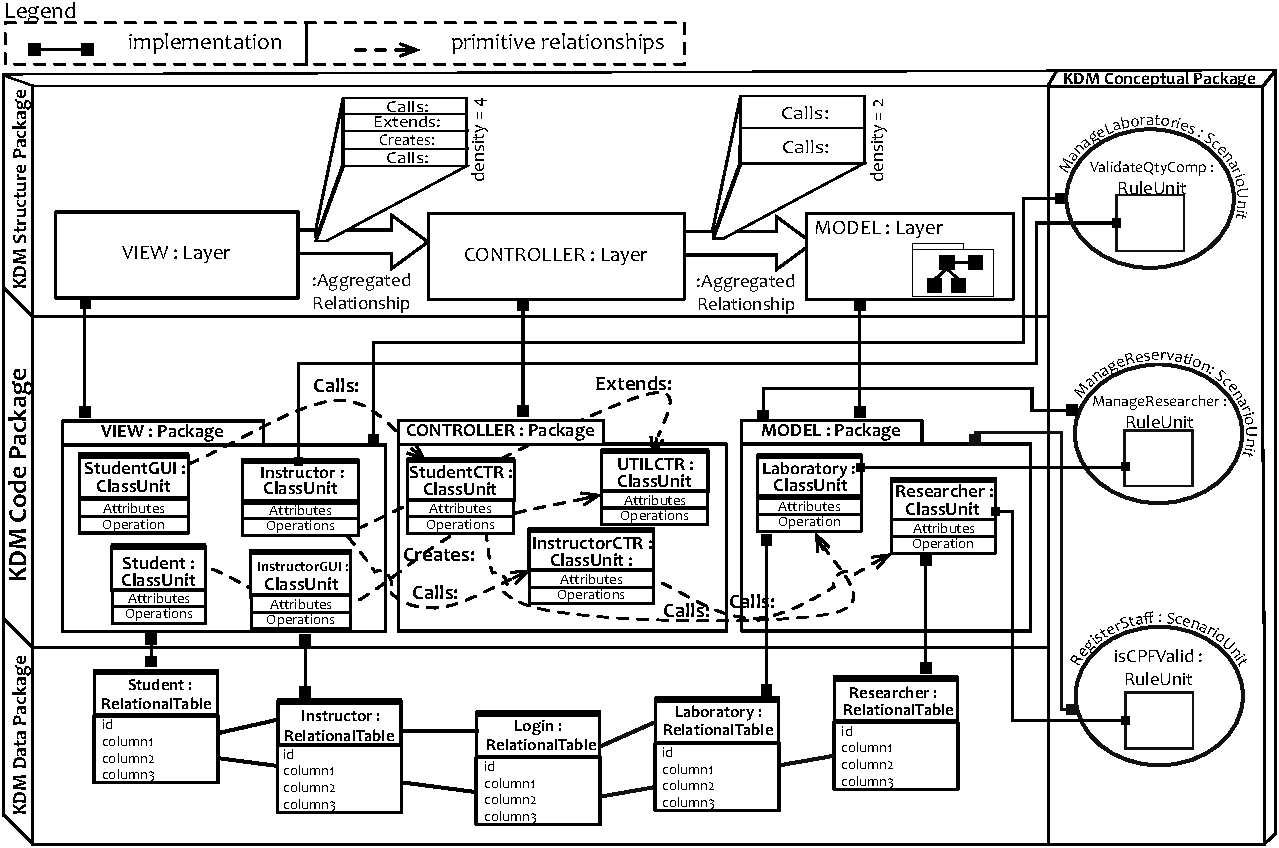
\includegraphics[scale=0.78]{figuras/NovoSystem6}
	\caption{Laboratory System (LabSys) depicted as an instance of KDM.}
	\label{fig:system}
\end{figure*}

ADM is the process of understanding  and evolving existing software systems taking model-driven principles into account~\cite{1686216}. A typical ADM process involves three main phases: Reverse Engineering, Refactorings/Optimizations, and Forward Engineering. In reverse engineering, a legacy system is abstracted in a KDM instance. Next, some refactorings and optimizations can be applied over the KDM instance and, in the last phase, the modernized source code is generated. 

KDM is the most important meta-model of ADM (ISO/IEC 19506), providing a comprehensive view of as-is application and data architectures, into a unique meta-model~\cite{Perez-Castillo:2011:KDM}. This is different from conventional model-driven development techniques we have found on literature~\cite{7051941}, since many of them employs several meta-models, from different vendors, along the process. KDM can be seen as a family of meta-models, as it contains twelve packages; each one representing a meta-model that concentrates on a different view of the system. Thus, by using its  meta-models, it is possible to have a number of views of a system. For example, it is possible to have a low level system representation, describing source-code details and several others views of the system, such as an architectural view, a data view, a business rule view, a behavioral view, etc. Moreover, as KDM groups a set of meta-models, all of them share the same terminology, i.e., all of the meta-models know the main meta-model elements, such as ClassUnit, KDMEntity and MethodUnit, etc.

Considering the scope of this paper, some important KDM packages are: Code, Structure, Data and Conceptual. Notice the slight difference between the terms ``view'' and ``package'' that we are using in this paper. For instance, herein using the KDM terminology, we can say the Code package allows the creation/existence of a view to represent the source code. Code package provides a lot of meta-classes for representing source code details, such as MethodUnit (methods), ClassUnit (classes) and StorableUnit (attributes). Structure package is devoted to represent the architecture of the system, employing architectural concepts commonly find in the literature. So, it offers meta-classes for representing layers (Layer meta-class), subsystems (Subsystem meta-class), components (Component meta-class) and architecture views (ArchitectureView meta-class). It also offers a special kind of relationship called AggregatedRelationhip meta-class, whose goal is to relate architectural elements with each other. An important characteristic of this relationship is that it acts as a container of primitive relationships, i.e., it is possible to group several primitive relationships within it. Data package represents the database structure of the system, providing meta-classes for representing tables and their attributes (Columns, primary key, etc). Conceptual package offers meta-classes for representing conceptual elements of a system, such as business rules (RuleUnit meta-class), scenarios (Scenario meta-class), etc. 

The KDM main goal is to allow a complete representation of systems, ranging from low to high-level views. All of the aforementioned meta-models, although being in different abstraction levels, can be interrelated to each other. For example, consider the existence of a Java package P1 (Package meta-class) that contains a class C1 (ClassUnit meta-class). This package can be the source-code realization of a Layer L1 (Layer meta-class) and, at the same time, the realization of a Scenario S1. The class C1 can also be the realization of a business rule B1 (RuleUnit meta-class) that is inside the scenario S1. 

\section{A Running Example}\label{sec:running_example}

Figure~\ref{fig:system} presents and describes an example that is used throughout this paper. It is shown schematically how KDM can be used for representing four abstractions views: Code View, Architecture View, Data View, and Conceptual View. We have used a real-life legacy information system named Laboratory System (LabSys), which is currently used by Federal University of Tocantins to control the use of laboratories in the entire university. This figure illustrates a KDM model, i.e., an instance of KDM composed by four KDM views/instances - each of the four big rectangles represents an instance of an internal meta-model. There is an instance of the Code meta-model (middle), an instance of the Structure meta-model (upper part), Data meta-model (lower part), and another one of the Conceptual meta-model (right part). 

Besides, each of the smaller internal elements (classes, packages, layers, relationships, etc) also contains instances of KDM meta-classes. Herein we use the pattern \textbf{``instance name: Meta-class name''} in the name of every element so that the name of the meta-class can be seen. As this is an MVC-based system, Code View contains three instances of the Package meta-class: VIEW, CONTROLLER, and MODEL. Each of them involves some ClassUnit instances. The classes are related to each other by means of static (associations, inheritance, interface realizations, etc) or dynamic (calls, object creation, parameter passing, etc) relationships. Each of these relationships is also an instance of specific meta-classes. 

The Architecture View represents the system architecture. In this example each smaller rectangle represents an instance of a meta-class called Layer. The system is organized in three layers:  VIEW, CONTROLLER, and MODEL. Between Layers and Packages there are a set of relationship called \texttt{implementation}, which are represented in Figure~\ref{fig:system} by the symbol \foobarMeu. The intention of this type of relationship is to denote that a specific higher-level abstraction is realized by one or more lower level code elements. In this example, the Layer VIEW is realized in source-code level by the Package VIEW; the Layer MODEL is realized by the Package MODEL and the Layer CONTROLLER by the Package CONTROLLER. The \texttt{implementation} relationship is very important in this work, as it is the main link between meta-models in different abstraction levels. Observe in the figure that the unique route between the views are by means of these relationships.
%
%KDM also possesses an important relationship type called AggregatedRelationship whose aim is to represent dependencies between architectural elements of the Structure Package. Using this relationship it is possible to put together several primitive relationships in a unique ``channel''. For example, there are thicker relationships between the layers representing the AggregatedRelationship. It is also possible to see that these relationships aggregate some primitive relationships. For example,

The thicker arrow ($\Rightarrow$) relationships between the layers represent an instance of AggregatedRelationship meta-class. The AggregatedRelationship between the Layer VIEW and the Layer CONTROLLER act as a ``channel'' to group primitive relationships, for instance: two Calls, one Creates and one Extends. The number aside the AggregatedRelationship is called ``density'' that represents the amount of primitive relationships exists inside it.

The Conceptual View illustrates the system's  business rules domain. This system owns three ScenarioUnits (ManageLaboratories, ManageReservation, and RegisterStaff), each of them are associated with a Package from Code View by means of the association \texttt{implementation}. Further, each ScenarioUnit contains a RuleUnit (ValidateQTYComputers, CheckCredentials, and isCPFValid, respectively) associated with a ClassUnit from Code View, again using the association implementation.

Finally, the Data View depicts the system's database and its tables. Notice that the depicted system owns a set of Plain Old Java Objects (POJOS), they are: Student, Instructor, Secretary, and Researcher. All of these POJOS are also Object Relational Mapping (ORM), i.e., they are mapped to the Data View using the meta-class RelationalTable and its columns are mapped using the meta-classes UniqueKey and ColumnSet.

Assuming the system as it is, it is possible to identify some flaws, i.e., classes that should be moved to another package, classes that are doing work that should be done by other class, a class is no longer used by system, etc. More information about these flaws are detailed and solved in the Case Study presented in Section~\ref{sec:case_study}.

%An evident problem in this AM system is the presence of the ClassUnits \texttt{Student} and \texttt{Instructor} in the VIEW package. A solution is to apply the \textit{Move Class} KDM refactoring as presented in Figure~\ref{fig:ATLRefactoring}.

%\begin{figure}[h]
%	\centering
	% Requires \usepackage{graphicx}
%	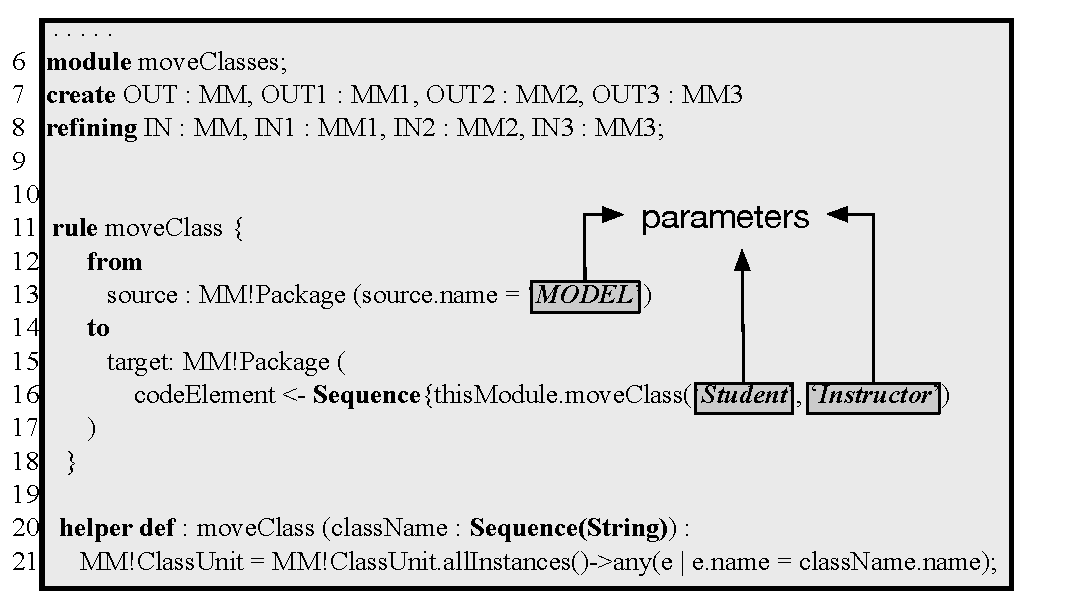
\includegraphics[scale=0.516]{figuras/NovoMoveClassFormatted}
%	\caption{Snippet of ATL to perform the refactoring \textit{Move Class}.}
%	\label{fig:ATLRefactoring}
%\end{figure}

%Lines 14 though 19 the \textit{Move Class} is actually defined. Lines 21 and 22 there is a helper, in ATL helpers are like methods in programing languages. This helper is used to verify if the ClassUnit is the correct class to be moved. 
%Almost all refactorings need some parameters that should be properly informed by the user. For instance, in Figure~\ref{fig:ATLRefactoring} lines 13 and 16 the software modernizer informed three parameters, i.e, he(she) specified the source Package (\texttt{MODEL}) and two ClassUnit's instances (\texttt{Student} and \texttt{Instructor}) to be moved. %that he(she) would like to move. After specifying these parameters the ATL is ready to be applied into a KDM instance.

%Observing the refactoring defined in Figure~\ref{fig:ATLRefactoring} it is fairly evident that both classes \texttt{Student} and \texttt{Instructor} should be moved to the MODEL package.
%
%During a refactoring activity, these classes should be moved to the Model package. 
%However, the effect of moving these ClassUnits will turn the KDM instance inconsistent, because the ``density'' value will turn wrong, i.e., AggregationRelationShip between the Layer VIEW and the Layer CONTROLLER would change from 4 to 2 - once the primitives relationships Creates and Extends would no longer exist from the package VIEW to the package CONTROLLER. In the same way, the result of \textit{Move Class} refactoring should also update the density between the Layer MODEL and CONTROLLER, instead of 2 it should be 4, as Creates and Extends were also moved along with its ClassUnits, \texttt{Student} and \texttt{Instructor}. Concerning to the Conceptual View, the RuleUnit \textit{CheckFreeHours} that is associated with \texttt{Instructor} should also be moved to ScenarioUnit \textit{RegisterStaff}.

%These propagation seen to be easy to apply, however, in a complex system comprising all KDM's packages/views propagate all changes, in a cascade way, after a refactoring is a difficult and error prone task. Even identifying the affected parts of the KDM's packages/views is not an easy and straightforward process. In order to fulfill this limitation and create a plug-in supported KDM-specific approach for updating dependent KDM models/views when specific elements are refactored.

%--------------valters background---------------------------------------




%----------------------------------------------------------------------

%In this section we provide a brief background to Architecture-Driven Modernization (ADM) and Knowledge Discovery Metamodel (KDM). 

%Further, we describe in detail why change propagation in KDM is a complex process.

%\subsection{ADM and KDM}

%The growing interest in using MDA to manage software evolution~\cite{Heckel2008, Andrade:2005, Reus:2006} 
%
%
%is mainly focused on the reengineering or modernization of legacy systems. Several software migration projects have been carried out with model-driven approaches~\cite{Heckel2008, Andrade:2005, Reus:2006}. %In addition, the 
%This interest 
%motived OMG to define the Architecture-Driven Modernization (ADM) initiative~\cite{1686216} which advocates carrying out the reengineering process considering models. 
%
%ADM is the concept of modernizing existing systems with a focus on all aspects of the current systems architecture and the ability to transform current architectures to target architectures by using all principles of MDD~\cite[p.~60]{Ulrich:2010:IST:1841736}. 
%
%
%Figure~\ref{fig:ADM_shorseshoe} depicts the horseshoe model (i.e., horseshoe is basically a left-hand side, a right-hand side and a bridge between the sides) adapted to ADM. %Please note that it contains all the traditional phases and some MDD's keywords, such as PSM and  PIM. The traditional phases adapted to ADM are:
%\begin{figure}[!ht]
%\centering
  % Requires \usepackage{graphicx}
% 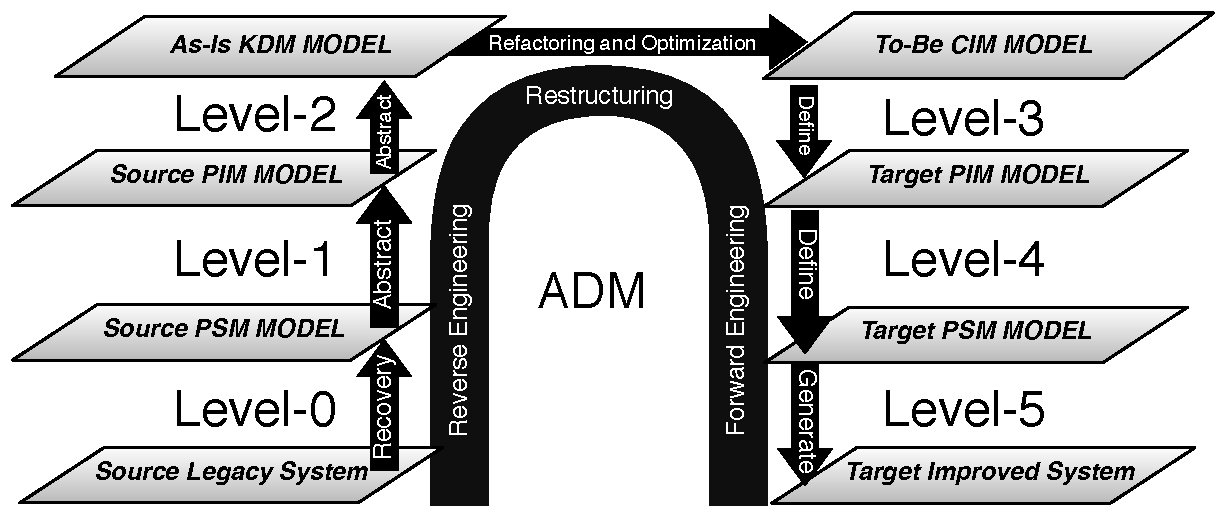
\includegraphics[scale=0.42]{figuras/processoDaFerramenta}
%\caption{Horseshoe Modernization Model~\cite{OMG_ADM}.}
%\label{fig:ADM_shorseshoe}
%\end{figure}
%This horseshoe model contains three main phases. The first one is the \textbf{Reverse Engineering} that takes a legacy system to be modernized as input.  Further the knowledge is extracted and a Platform-Specific Model (PSM) is generated. Next, this PSM serves as the basis for the generation of a Platform-Independent Language (PIM), which is called KDM. The second phase is the \textbf{Restructuring}, in which a set set of reengineering/refactoring can be applied into a KDM's instance by means of model transformations. The third phase is the \textbf{Forward Engineering} where a forward engineering is carried out and the source code of the modernized target system is generated.

%Figure~\ref{horseshoe} depicts the ADM modernization domain model where the left side of the horseshoe is the current state of a busines/it architecture ``as is'' and the right side is what we want to get after the modernization ``to-be''. %One common path followed by IT is to focus on the technical architecture. Generally, the cost of this approach is lower and project duration shorter because the data and application architectures remain largely intact but there is almost no impact or value to the business. 

%On the other hand, a modernization which seeks to provide value to the business, would need to change the application and data architecture, which in turn would rely on an analysis of requirements stemming from shifts to the business architecture. These types of projects are of a longer duration, require more investment, and deliver significantly more value to the business.




%To perform a systematic modernization as depicted in Figure~\ref{fig:ADM_shorseshoe}, ADM introduces several modernization standards, among them there is the Knowledge Discovery Metamodel (KDM).
%However, herein we focus on KDM because it is the key cornerstone of ADM and the main ideas of our research.  KDM is an OMG specification adopted as ISO/IEC 19506 by the International Standards Organization for representing information related to existing software systems. The goal of the KDM standard is to define a metamodel to represent all the different legacy software artifacts involved in a legacy information system (e.g. Code, Architecture, Business Rules, Data, Events, etc.). %The metamodel of the KDM standard provides a comprehensive high-level view of the behavior, structure and data of legacy information systems by means of a set of facts. 

%KDM contains twelve packages and it is structured in a hierarchy of four layers: (\textit{i}) Infrastructure Layer, (\textit{ii}) Program Elements Layer, (\textit{iii}) Runtime Resource Layer, and (\textit{iv}) Abstractions Layer. These layers can be instantiated automatically, semi-automatically or manually through the application of various techniques of extraction of knowledge, analysis and transformations~\cite{1686216}. Figure~\ref{fig:kdmLayers} depicts the architecture of KDM and its layers. %By observing this figure it is fairly evident that each layer is based on the previous layer. 
%They are organized into packages that define a set of metamodel, whose purpose is to represent a specific and independent interest of knowledge related to legacy systems, e.g. source code, user interfaces, databases, business rules, etc.

%\begin{figure}[!ht]
%\centering
  % Requires \usepackage{graphicx}
 %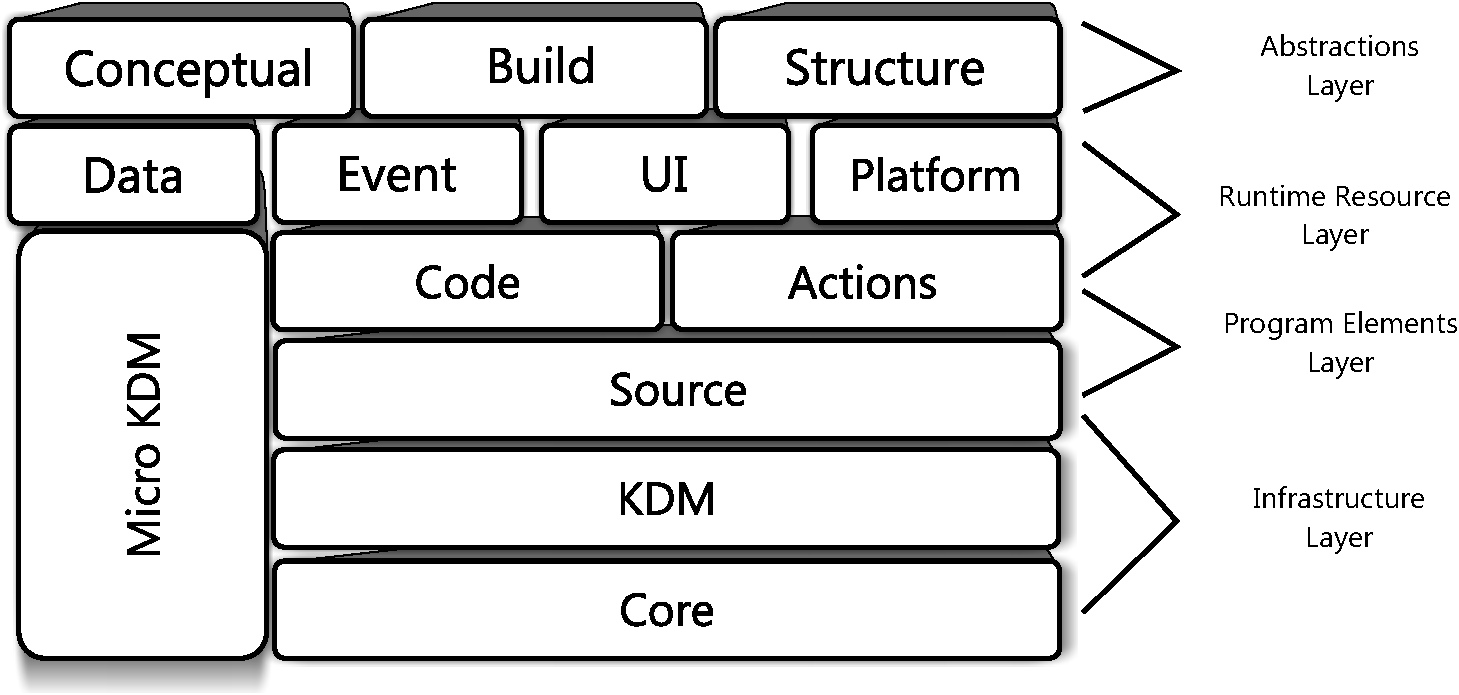
\includegraphics[width=3.3in]{figuras/camadas_kdm}
%\caption{KDM Architecture.}
%\label{fig:kdmLayers}
%\end{figure}

%Although KDM is a metamodel to represent a whole system, its main purpose is not the representation of models related strictly to the source code nature such as Unified Modeling Language (UML). While UML can be used to generate new code in a top-down manner, an ADM-based process using KDM starts from the different legacy software artifacts and builds higher-abstraction level models in a bottom-up manner through reverse engineering techniques. %KDM can be seen from different perspectives, as follows: (\textit{i}) KDM can be considered as a metamodel to represent legacy knowledge models, (\textit{ii}) most of the KDM specification is a definition of a language- and platform-independent ontology of legacy information systems and (\textit{iii}) KDM is a common interchange format that makes the interoperability between the reverse engineering tools and modernization tools possible.

%KDM specification owns some KDM domain, each domain defines an architectural viewpoint. In order to define the catalogue of refactoring for the KDM we need to focus just on the Program Element Layer - more specifically  in the Code Package, which represents the code elements of a program (classes, fields and methods) and their associations. %We are interested in the Code Package once our catalogue is based on fine-grained refactorings, i.e., refactorings to be applied into classes, fields and methods. 
%Therefore, it is important to dig a little deeper in the Code Package.
%
%In a given KDM instance, each instance of the code meta-model element represents some programming language construct, determined by the programming language of the existing software system. Each instance of a code meta-model element corresponds to a certain region of the source code in one of the artifacts of the existing software system. In addition, 
%
%The Code Package consists of $24$ classes and contains all the abstract elements for modeling the static structure of the source code. In Table~\ref{tab:mappingCodeToKDM} is depicted some of them. This table identifies KDM metaclasses possessing similar characteristics to the static structure of the source code. Some metaclasses can be direct mapped, such as Class from object-oriented language, which can be easily mapped to the ClassUnit metaclass from KDM.


%\begin{table}[!h]
%\caption{Metaclasses for modeling the static structure of the source-code}
%\label{tab:mappingCodeToKDM}
%\centering
%\begin{tabular}{|>{\centering}p{3cm}|>{\centering}p{3cm}|}
%\hline 
%Source-Code Element & KDM Element\tabularnewline
%\hline 
%\hline 
%Class & ClassUnit\tabularnewline
%\hline 
%Interface & InterfaceUnit\tabularnewline
%\hline 
%Method & MethodUnit\tabularnewline
%\hline 
%Field & StorableUnit\tabularnewline
%\hline 
%Local Variable & Member\tabularnewline
%\hline 
%Parameter & ParameterUnit\tabularnewline
%\hline 
%Association & KDM RelationShip\tabularnewline
%\hline 
%\end{tabular}
%\end{table}

  %\begin{figure}[!ht]
  %\centering
  % Requires \usepackage{graphicx}
    %\includegraphics[scale=0.39]{FIGURAS_DA_REFATORACAO/ProgramLaye0r}
  %\caption{Chunk of the Code Package (OMG Group~\cite{OMGADM})}
  %\label{fig:programLayer}
  %\end{figure}

 %As can be seen in Figure~\ref{fig:programLayer} the root metaclass is \textit{ComputationalObject} which has two sub-metaclasses, i.e., \textit{DataElement} and \textit{ControlElement}. The former sub-metaclass, \textit{DataElement}, is a generic modeling element that defines the common properties of several concrete classes that represent the named data items of existing software systems, for example, global and local variables, record files, and formal parameters. \textit{DataElement} has five sub-metaclasses - \textit{StorableUnit}, \textit{IndexUnit}, \textit{ItemUnit}, \textit{ParameterUnit} and \textit{MemberUnit}. \textit{StorableUnit} is a concrete  sub-metaclass of the \textit{StorableElement} meta-class that represents variables of the existing software system. \textit{IndexUnit} class is a concrete subclass of the \textit{DataElement} class that represents an index of an array datatype. Instances of \textit{ItemUnit} class are endpoints of KDM data relations which describes access to complex datatypes. \textit{ParameterUnit} class is a concrete subclass of the \textit{DataElement} class that represents a formal parameter; for example, a formal parameter of a procedure. \textit{MemberUnit} class is a concrete subclass of the \textit{DataElement} class that represents a member of a class type. Finally, the latter, \textit{ControlElement} is a sub-metaclass that contains two sub-metaclasses - \textit{MethodUnit} and \textit{CallableUnit}. \textit{MethodUnit} element represents member functions owned by a \textit{ClassUnit}, including user-defined operators, constructors and destructors. The \textit{CallableUnit} represents a basic stand-alone element that can be called, such as a procedure or a function. %As can be seen below the dashed line in Figure~\ref{fig:programLayer} there are also the following enumerations: ``\textit{ExportKind}'', ``\textit{StorableKind}'', ``\textit{CallableKind}'', ``\textit{MethodKind}'', which are sets os literals used as properties of the metaclasses.


